\documentclass[]{article}
\usepackage{lmodern}
\usepackage{amssymb,amsmath}
\usepackage{ifxetex,ifluatex}
\usepackage{fixltx2e} % provides \textsubscript
\ifnum 0\ifxetex 1\fi\ifluatex 1\fi=0 % if pdftex
  \usepackage[T1]{fontenc}
  \usepackage[utf8]{inputenc}
\else % if luatex or xelatex
  \ifxetex
    \usepackage{mathspec}
  \else
    \usepackage{fontspec}
  \fi
  \defaultfontfeatures{Ligatures=TeX,Scale=MatchLowercase}
\fi
% use upquote if available, for straight quotes in verbatim environments
\IfFileExists{upquote.sty}{\usepackage{upquote}}{}
% use microtype if available
\IfFileExists{microtype.sty}{%
\usepackage{microtype}
\UseMicrotypeSet[protrusion]{basicmath} % disable protrusion for tt fonts
}{}
\usepackage[margin=1in]{geometry}
\usepackage{hyperref}
\hypersetup{unicode=true,
            pdftitle={Mineração de texto em pedidos de Lei de Acesso ä informação - LAI},
            pdfborder={0 0 0},
            breaklinks=true}
\urlstyle{same}  % don't use monospace font for urls
\usepackage{color}
\usepackage{fancyvrb}
\newcommand{\VerbBar}{|}
\newcommand{\VERB}{\Verb[commandchars=\\\{\}]}
\DefineVerbatimEnvironment{Highlighting}{Verbatim}{commandchars=\\\{\}}
% Add ',fontsize=\small' for more characters per line
\usepackage{framed}
\definecolor{shadecolor}{RGB}{248,248,248}
\newenvironment{Shaded}{\begin{snugshade}}{\end{snugshade}}
\newcommand{\KeywordTok}[1]{\textcolor[rgb]{0.13,0.29,0.53}{\textbf{#1}}}
\newcommand{\DataTypeTok}[1]{\textcolor[rgb]{0.13,0.29,0.53}{#1}}
\newcommand{\DecValTok}[1]{\textcolor[rgb]{0.00,0.00,0.81}{#1}}
\newcommand{\BaseNTok}[1]{\textcolor[rgb]{0.00,0.00,0.81}{#1}}
\newcommand{\FloatTok}[1]{\textcolor[rgb]{0.00,0.00,0.81}{#1}}
\newcommand{\ConstantTok}[1]{\textcolor[rgb]{0.00,0.00,0.00}{#1}}
\newcommand{\CharTok}[1]{\textcolor[rgb]{0.31,0.60,0.02}{#1}}
\newcommand{\SpecialCharTok}[1]{\textcolor[rgb]{0.00,0.00,0.00}{#1}}
\newcommand{\StringTok}[1]{\textcolor[rgb]{0.31,0.60,0.02}{#1}}
\newcommand{\VerbatimStringTok}[1]{\textcolor[rgb]{0.31,0.60,0.02}{#1}}
\newcommand{\SpecialStringTok}[1]{\textcolor[rgb]{0.31,0.60,0.02}{#1}}
\newcommand{\ImportTok}[1]{#1}
\newcommand{\CommentTok}[1]{\textcolor[rgb]{0.56,0.35,0.01}{\textit{#1}}}
\newcommand{\DocumentationTok}[1]{\textcolor[rgb]{0.56,0.35,0.01}{\textbf{\textit{#1}}}}
\newcommand{\AnnotationTok}[1]{\textcolor[rgb]{0.56,0.35,0.01}{\textbf{\textit{#1}}}}
\newcommand{\CommentVarTok}[1]{\textcolor[rgb]{0.56,0.35,0.01}{\textbf{\textit{#1}}}}
\newcommand{\OtherTok}[1]{\textcolor[rgb]{0.56,0.35,0.01}{#1}}
\newcommand{\FunctionTok}[1]{\textcolor[rgb]{0.00,0.00,0.00}{#1}}
\newcommand{\VariableTok}[1]{\textcolor[rgb]{0.00,0.00,0.00}{#1}}
\newcommand{\ControlFlowTok}[1]{\textcolor[rgb]{0.13,0.29,0.53}{\textbf{#1}}}
\newcommand{\OperatorTok}[1]{\textcolor[rgb]{0.81,0.36,0.00}{\textbf{#1}}}
\newcommand{\BuiltInTok}[1]{#1}
\newcommand{\ExtensionTok}[1]{#1}
\newcommand{\PreprocessorTok}[1]{\textcolor[rgb]{0.56,0.35,0.01}{\textit{#1}}}
\newcommand{\AttributeTok}[1]{\textcolor[rgb]{0.77,0.63,0.00}{#1}}
\newcommand{\RegionMarkerTok}[1]{#1}
\newcommand{\InformationTok}[1]{\textcolor[rgb]{0.56,0.35,0.01}{\textbf{\textit{#1}}}}
\newcommand{\WarningTok}[1]{\textcolor[rgb]{0.56,0.35,0.01}{\textbf{\textit{#1}}}}
\newcommand{\AlertTok}[1]{\textcolor[rgb]{0.94,0.16,0.16}{#1}}
\newcommand{\ErrorTok}[1]{\textcolor[rgb]{0.64,0.00,0.00}{\textbf{#1}}}
\newcommand{\NormalTok}[1]{#1}
\usepackage{graphicx,grffile}
\makeatletter
\def\maxwidth{\ifdim\Gin@nat@width>\linewidth\linewidth\else\Gin@nat@width\fi}
\def\maxheight{\ifdim\Gin@nat@height>\textheight\textheight\else\Gin@nat@height\fi}
\makeatother
% Scale images if necessary, so that they will not overflow the page
% margins by default, and it is still possible to overwrite the defaults
% using explicit options in \includegraphics[width, height, ...]{}
\setkeys{Gin}{width=\maxwidth,height=\maxheight,keepaspectratio}
\IfFileExists{parskip.sty}{%
\usepackage{parskip}
}{% else
\setlength{\parindent}{0pt}
\setlength{\parskip}{6pt plus 2pt minus 1pt}
}
\setlength{\emergencystretch}{3em}  % prevent overfull lines
\providecommand{\tightlist}{%
  \setlength{\itemsep}{0pt}\setlength{\parskip}{0pt}}
\setcounter{secnumdepth}{0}
% Redefines (sub)paragraphs to behave more like sections
\ifx\paragraph\undefined\else
\let\oldparagraph\paragraph
\renewcommand{\paragraph}[1]{\oldparagraph{#1}\mbox{}}
\fi
\ifx\subparagraph\undefined\else
\let\oldsubparagraph\subparagraph
\renewcommand{\subparagraph}[1]{\oldsubparagraph{#1}\mbox{}}
\fi

%%% Use protect on footnotes to avoid problems with footnotes in titles
\let\rmarkdownfootnote\footnote%
\def\footnote{\protect\rmarkdownfootnote}

%%% Change title format to be more compact
\usepackage{titling}

% Create subtitle command for use in maketitle
\newcommand{\subtitle}[1]{
  \posttitle{
    \begin{center}\large#1\end{center}
    }
}

\setlength{\droptitle}{-2em}

  \title{Mineração de texto em pedidos de Lei de Acesso ä informação - LAI}
    \pretitle{\vspace{\droptitle}\centering\huge}
  \posttitle{\par}
    \author{}
    \preauthor{}\postauthor{}
    \date{}
    \predate{}\postdate{}
  
\usepackage{booktabs}
\usepackage{longtable}
\usepackage{array}
\usepackage{multirow}
\usepackage[table]{xcolor}
\usepackage{wrapfig}
\usepackage{float}
\usepackage{colortbl}
\usepackage{pdflscape}
\usepackage{tabu}
\usepackage{threeparttable}
\usepackage{threeparttablex}
\usepackage[normalem]{ulem}
\usepackage{makecell}

\begin{document}
\maketitle

\subsection{Packages for this routine}\label{packages-for-this-routine}

\subsection{Importação e preparação dos
dados}\label{importacao-e-preparacao-dos-dados}

\subsubsection{Pedidos e-SIC}\label{pedidos-e-sic}

\begin{Shaded}
\begin{Highlighting}[]
\NormalTok{PATH =}\StringTok{ "C:/proj_eSIC_v10/textmining_pt/DATA/"}
\CommentTok{#PATH = "/Users/ewersonpimenta/Desktop/ESIC_TCC/Pedidos_LAI_EPE/BASE_DADOS/"}
\NormalTok{FILE =}\StringTok{ "relatorio_pedidos.ods"}
\NormalTok{db_raw =}\StringTok{ }\NormalTok{readODS}\OperatorTok{::}\KeywordTok{read.ods}\NormalTok{(}\DataTypeTok{file =} \KeywordTok{paste0}\NormalTok{(PATH,FILE), }\DataTypeTok{sheet =} \DecValTok{1}\NormalTok{); }\CommentTok{# dim(db_raw)}
\NormalTok{dbnames =}\StringTok{ }\NormalTok{db_raw[}\DecValTok{1}\NormalTok{,]; db_raw =}\StringTok{ }\NormalTok{db_raw[}\OperatorTok{-}\DecValTok{1}\NormalTok{,]; }
\KeywordTok{colnames}\NormalTok{(db_raw) =}\StringTok{ }\KeywordTok{c}\NormalTok{(}\StringTok{"ID"}\NormalTok{, }\StringTok{"DATA_PEDIDO"}\NormalTok{, }\StringTok{"DATA_PRAZOATEND"}\NormalTok{, }\StringTok{"DESCRI_PEDIDO"}\NormalTok{,}
                     \StringTok{"RESUMO_PEDIDO"}\NormalTok{, }\StringTok{"DATA_RESPOSTA"}\NormalTok{)}
\CommentTok{#View(head(db_raw))}
\NormalTok{LAI =}\StringTok{ }\NormalTok{db_raw}
\end{Highlighting}
\end{Shaded}

\subsubsection{Respostas e-SIC}\label{respostas-e-sic}

\begin{Shaded}
\begin{Highlighting}[]
\NormalTok{FILE1 =}\StringTok{ "relatorio_respostas.xlsx"}
\NormalTok{db1_raw =}\StringTok{ }\NormalTok{readxl}\OperatorTok{::}\KeywordTok{read_excel}\NormalTok{(}\KeywordTok{paste0}\NormalTok{(PATH,FILE1), }\DataTypeTok{sheet =} \StringTok{"DADOS"}\NormalTok{, }\DataTypeTok{col_names =} \OtherTok{TRUE}\NormalTok{); }
\CommentTok{# dim(db1_raw); names(db1_raw)}
\KeywordTok{colnames}\NormalTok{(db1_raw) =}\StringTok{ }\KeywordTok{c}\NormalTok{(}\StringTok{"ID"}\NormalTok{, }\StringTok{"DATA"}\NormalTok{, }\StringTok{"SOLICITACAO"}\NormalTok{, }\StringTok{"DIRETORIA"}\NormalTok{, }\StringTok{"DATA_RESPOSTA"}\NormalTok{)}
\CommentTok{#View(head(db1_raw))}
\NormalTok{LAI1 =}\StringTok{ }\NormalTok{db1_raw}
\end{Highlighting}
\end{Shaded}

\paragraph{Freq. de solicitações no e-SIC por Diretoria da
EPE}\label{freq.-de-solicitacoes-no-e-sic-por-diretoria-da-epe}

\begin{Shaded}
\begin{Highlighting}[]
\NormalTok{LAI1 }\OperatorTok
\StringTok{ }\KeywordTok{count}\NormalTok{(DIRETORIA, }\DataTypeTok{sort =} \OtherTok{TRUE}\NormalTok{) }\OperatorTok
\StringTok{  }\KeywordTok{kable}\NormalTok{(}\StringTok{"latex"}\NormalTok{, }\DataTypeTok{caption =} \StringTok{"Frequência de solicitações e-SIC por Diretoria/EPE"}\NormalTok{,}
        \DataTypeTok{booktabs =}\NormalTok{ T) }\OperatorTok
\StringTok{  }\KeywordTok{kable_styling}\NormalTok{(}\DataTypeTok{latex_options =} \KeywordTok{c}\NormalTok{(}\StringTok{"striped"}\NormalTok{, }\StringTok{"hold_position"}\NormalTok{))}
\end{Highlighting}
\end{Shaded}

\rowcolors{2}{gray!6}{white}

\begin{table}[!h]

\caption{\label{tab:unnamed-chunk-4}Frequência de solicitações e-SIC por Diretoria/EPE}
\centering
\begin{tabular}[t]{lr}
\hiderowcolors
\toprule
DIRETORIA & n\\
\midrule
\showrowcolors
DEA & 210\\
DEE & 197\\
DGC & 115\\
DPG & 24\\
OUTROS & 19\\
SIC & 1\\
\bottomrule
\end{tabular}
\end{table}

\rowcolors{2}{white}{white}

\paragraph{Respostas e-SIC - Reclassificação
Diretorias}\label{respostas-e-sic---reclassificacao-diretorias}

\begin{Shaded}
\begin{Highlighting}[]
\NormalTok{diretorias =}\StringTok{ }\KeywordTok{levels}\NormalTok{(}\KeywordTok{as.factor}\NormalTok{(LAI1}\OperatorTok{$}\NormalTok{DIRETORIA))}
\NormalTok{LAI1 =}\StringTok{ }\NormalTok{LAI1 }\OperatorTok\StringTok{ }
\StringTok{  }\KeywordTok{mutate}\NormalTok{(}\DataTypeTok{DIRETORIA =} \KeywordTok{ifelse}\NormalTok{(DIRETORIA }\OperatorTok{==}\StringTok{ }\NormalTok{diretorias[}\DecValTok{6}\NormalTok{],diretorias[}\DecValTok{5}\NormalTok{],DIRETORIA))}
\NormalTok{diretorias =}\StringTok{ }\KeywordTok{levels}\NormalTok{(}\KeywordTok{as.factor}\NormalTok{(LAI1}\OperatorTok{$}\NormalTok{DIRETORIA))}
\NormalTok{LAI1 =}\StringTok{ }\NormalTok{LAI1 }\OperatorTok\StringTok{ }
\StringTok{  }\KeywordTok{mutate}\NormalTok{(}\DataTypeTok{DIR_NEW =} \KeywordTok{ifelse}\NormalTok{(DIRETORIA }\OperatorTok{==}\StringTok{ }\NormalTok{diretorias[}\DecValTok{1}\NormalTok{],diretorias[}\DecValTok{1}\NormalTok{],}
                          \KeywordTok{ifelse}\NormalTok{(DIRETORIA }\OperatorTok{==}\StringTok{ }\NormalTok{diretorias[}\DecValTok{2}\NormalTok{],diretorias[}\DecValTok{2}\NormalTok{], }\StringTok{"OUTRAS"}\NormalTok{)))}
\CommentTok{#dim(LAI1)}
\CommentTok{#View(head(LAI1))}
\end{Highlighting}
\end{Shaded}

\begin{Shaded}
\begin{Highlighting}[]
\NormalTok{LAI1 }\OperatorTok
\StringTok{ }\KeywordTok{count}\NormalTok{(DIRETORIA, }\DataTypeTok{sort =} \OtherTok{TRUE}\NormalTok{) }\OperatorTok
\StringTok{  }\KeywordTok{kable}\NormalTok{(}\StringTok{"latex"}\NormalTok{, }\DataTypeTok{caption =} \StringTok{"Frequência de solicitações e-SIC por Diretoria/EPE - sem SIC"}\NormalTok{, }
        \DataTypeTok{booktabs =}\NormalTok{ T) }\OperatorTok
\StringTok{  }\KeywordTok{kable_styling}\NormalTok{(}\DataTypeTok{latex_options =} \KeywordTok{c}\NormalTok{(}\StringTok{"striped"}\NormalTok{, }\StringTok{"hold_position"}\NormalTok{))}
\end{Highlighting}
\end{Shaded}

\rowcolors{2}{gray!6}{white}

\begin{table}[!h]

\caption{\label{tab:unnamed-chunk-6}Frequência de solicitações e-SIC por Diretoria/EPE - sem SIC}
\centering
\begin{tabular}[t]{lr}
\hiderowcolors
\toprule
DIRETORIA & n\\
\midrule
\showrowcolors
DEA & 210\\
DEE & 197\\
DGC & 115\\
DPG & 24\\
OUTROS & 20\\
\bottomrule
\end{tabular}
\end{table}

\rowcolors{2}{white}{white}

\begin{Shaded}
\begin{Highlighting}[]
\NormalTok{LAI1 }\OperatorTok
\StringTok{ }\KeywordTok{count}\NormalTok{(DIR_NEW, }\DataTypeTok{sort =} \OtherTok{TRUE}\NormalTok{) }\OperatorTok
\StringTok{  }\KeywordTok{kable}\NormalTok{(}\StringTok{"latex"}\NormalTok{, }\DataTypeTok{caption =} \StringTok{"Frequência de solicitações e-SIC por Diretoria/EPE (TOP2)"}\NormalTok{,}
        \DataTypeTok{booktabs =}\NormalTok{ T) }\OperatorTok
\StringTok{  }\KeywordTok{kable_styling}\NormalTok{(}\DataTypeTok{latex_options =} \KeywordTok{c}\NormalTok{(}\StringTok{"striped"}\NormalTok{, }\StringTok{"hold_position"}\NormalTok{))}
\end{Highlighting}
\end{Shaded}

\rowcolors{2}{gray!6}{white}

\begin{table}[!h]

\caption{\label{tab:unnamed-chunk-7}Frequência de solicitações e-SIC por Diretoria/EPE (TOP2)}
\centering
\begin{tabular}[t]{lr}
\hiderowcolors
\toprule
DIR\_NEW & n\\
\midrule
\showrowcolors
DEA & 210\\
DEE & 197\\
OUTRAS & 159\\
\bottomrule
\end{tabular}
\end{table}

\rowcolors{2}{white}{white}

\subsubsection{Unificando as duas bases}\label{unificando-as-duas-bases}

\begin{Shaded}
\begin{Highlighting}[]
\NormalTok{LAI =}\StringTok{ }\NormalTok{LAI }\OperatorTok\StringTok{ }\KeywordTok{select}\NormalTok{(}\OperatorTok{-}\NormalTok{DATA_RESPOSTA); }\CommentTok{#dim(LAI)}
\NormalTok{LAI1 =}\StringTok{ }\NormalTok{LAI1 }\OperatorTok\StringTok{ }\KeywordTok{select}\NormalTok{(}\OperatorTok{-}\NormalTok{DATA); }\CommentTok{#dim(LAI1)}
\NormalTok{DB =}\StringTok{ }\KeywordTok{left_join}\NormalTok{(}\DataTypeTok{x =}\NormalTok{ LAI, }\DataTypeTok{y =}\NormalTok{ LAI1, }\DataTypeTok{by =} \StringTok{"ID"}\NormalTok{)}
\CommentTok{#View(head(DB))}
\NormalTok{DB[}\KeywordTok{c}\NormalTok{(}\DecValTok{32}\NormalTok{,}\DecValTok{50}\NormalTok{,}\DecValTok{66}\NormalTok{),}\KeywordTok{c}\NormalTok{(}\OperatorTok{-}\DecValTok{1}\NormalTok{,}\OperatorTok{-}\DecValTok{3}\NormalTok{,}\OperatorTok{-}\DecValTok{5}\NormalTok{,}\OperatorTok{-}\DecValTok{6}\NormalTok{,}\OperatorTok{-}\DecValTok{9}\NormalTok{)] }\OperatorTok
\StringTok{  }\KeywordTok{select}\NormalTok{(DATA_PEDIDO, DATA_RESPOSTA, DIRETORIA, DESCRI_PEDIDO) }\OperatorTok
\KeywordTok{kable}\NormalTok{(}\StringTok{"latex"}\NormalTok{, }\DataTypeTok{caption =} \StringTok{"Amostra dos dados a serem pré-processados"}\NormalTok{, }\DataTypeTok{booktabs =}\NormalTok{ T) }\OperatorTok
\StringTok{  }\KeywordTok{kable_styling}\NormalTok{(}\DataTypeTok{latex_options =} \KeywordTok{c}\NormalTok{(}\StringTok{"striped"}\NormalTok{, }\StringTok{"hold_position"}\NormalTok{), }\DataTypeTok{full_width =}\NormalTok{ F) }\OperatorTok
\StringTok{  }\KeywordTok{column_spec}\NormalTok{(}\DecValTok{4}\OperatorTok{:}\DecValTok{4}\NormalTok{, }\DataTypeTok{width =} \StringTok{"2cm"}\NormalTok{) }\OperatorTok
\StringTok{  }\KeywordTok{column_spec}\NormalTok{(}\DecValTok{5}\OperatorTok{:}\DecValTok{5}\NormalTok{, }\DataTypeTok{width =} \StringTok{"10cm"}\NormalTok{) }\OperatorTok
\KeywordTok{landscape}\NormalTok{()}
\end{Highlighting}
\end{Shaded}

\begin{landscape}\rowcolors{2}{gray!6}{white}
\begin{table}[!h]

\caption{\label{tab:unnamed-chunk-8}Amostra dos dados a serem pré-processados}
\centering
\begin{tabular}[t]{lll>{\raggedright\arraybackslash}p{2cm}>{\raggedright\arraybackslash}p{10cm}}
\hiderowcolors
\toprule
  & DATA\_PEDIDO & DATA\_RESPOSTA & DIRETORIA & DESCRI\_PEDIDO\\
\midrule
\showrowcolors
32 & 30/08/2018 16:44 & 2018-08-31 & DEA & Boa tarde, 

Gostaria de solicitar os dados históricos de Estatísticas do Consumo de Energia Elétrica (GWh), divulgados pela ONS na Resenha Mensal. 

A finalidade é estudo econométrico da série histórica de consumo de energia no Brasil e nos setores da economia. 

Obrigada.\\
50 & 25/08/2015 18:35 & 2015-09-04 & DEE & Prezados, boa tarde!

Solicito a cópia da NT EPE-DEE-RE-077/2008.

Estou realizando alguns estudos pertinentes a CUR e preciso deste arquivo de referência.

Grato pela atenção!

Thiago Paulino\\
66 & 21/10/2015 14:53 & 2015-10-26 & DEE & Prezados, bom dia!

Sirvo-me do presente para solicitar o COP CEC - Suape II - Leilão 01/2007.\\
\bottomrule
\end{tabular}
\end{table}
\rowcolors{2}{white}{white}
\end{landscape}

\subsubsection{Análise de texto}\label{analise-de-texto}

\paragraph{Frequência de palavras por
diretoria}\label{frequencia-de-palavras-por-diretoria}

\begin{Shaded}
\begin{Highlighting}[]
\NormalTok{diretoria_palavras <-}\StringTok{ }\NormalTok{DB }\OperatorTok
\StringTok{  }\KeywordTok{unnest_tokens}\NormalTok{(palavra, DESCRI_PEDIDO) }\OperatorTok
\StringTok{  }\KeywordTok{count}\NormalTok{(DIRETORIA, palavra, }\DataTypeTok{sort =} \OtherTok{TRUE}\NormalTok{) }\OperatorTok
\StringTok{  }\KeywordTok{ungroup}\NormalTok{()}
\CommentTok{#diretoria_palavras}

\NormalTok{plot_diretoria_palavras <-}\StringTok{ }\NormalTok{diretoria_palavras }\OperatorTok
\StringTok{  }\KeywordTok{bind_tf_idf}\NormalTok{(palavra, DIRETORIA, n) }\OperatorTok
\StringTok{  }\KeywordTok{arrange}\NormalTok{(}\KeywordTok{desc}\NormalTok{(tf_idf)) }\OperatorTok
\StringTok{  }\KeywordTok{mutate}\NormalTok{(}\DataTypeTok{palavra =} \KeywordTok{factor}\NormalTok{(palavra, }\DataTypeTok{levels =} \KeywordTok{rev}\NormalTok{(}\KeywordTok{unique}\NormalTok{(palavra)))) }\OperatorTok
\StringTok{  }\KeywordTok{mutate}\NormalTok{(}\DataTypeTok{DIRETORIA =} \KeywordTok{factor}\NormalTok{(DIRETORIA, }\DataTypeTok{levels =} \KeywordTok{c}\NormalTok{(}\StringTok{"DEA"}\NormalTok{,}
                                                  \StringTok{"DEE"}\NormalTok{,}
                                                  \StringTok{"DGC"}\NormalTok{,}
                                                  \StringTok{"DPG"}\NormalTok{,}
                                                  \StringTok{"OUTROS"}\NormalTok{)))}
\CommentTok{#View(head(plot_diretoria_palavras))}
\CommentTok{#jpeg("02_freq_palavras_dir.jpeg")}
\NormalTok{plot_diretoria_palavras }\OperatorTok
\KeywordTok{group_by}\NormalTok{(DIRETORIA) }\OperatorTok
\KeywordTok{top_n}\NormalTok{(}\DecValTok{10}\NormalTok{, tf_idf) }\OperatorTok
\KeywordTok{ungroup}\NormalTok{() }\OperatorTok
\KeywordTok{mutate}\NormalTok{(}\DataTypeTok{palavra =} \KeywordTok{reorder}\NormalTok{(palavra, tf_idf)) }\OperatorTok
\KeywordTok{ggplot}\NormalTok{(}\KeywordTok{aes}\NormalTok{(palavra, tf_idf, }\DataTypeTok{fill =}\NormalTok{ DIRETORIA)) }\OperatorTok{+}
\KeywordTok{geom_col}\NormalTok{(}\DataTypeTok{show.legend =} \OtherTok{FALSE}\NormalTok{) }\OperatorTok{+}
\KeywordTok{labs}\NormalTok{(}\DataTypeTok{x =} \OtherTok{NULL}\NormalTok{, }\DataTypeTok{y =} \StringTok{"tf-idf"}\NormalTok{) }\OperatorTok{+}
\KeywordTok{facet_wrap}\NormalTok{(}\OperatorTok{~}\NormalTok{DIRETORIA, }\DataTypeTok{ncol =} \DecValTok{2}\NormalTok{, }\DataTypeTok{scales =} \StringTok{"free"}\NormalTok{) }\OperatorTok{+}
\KeywordTok{coord_flip}\NormalTok{()}
\end{Highlighting}
\end{Shaded}

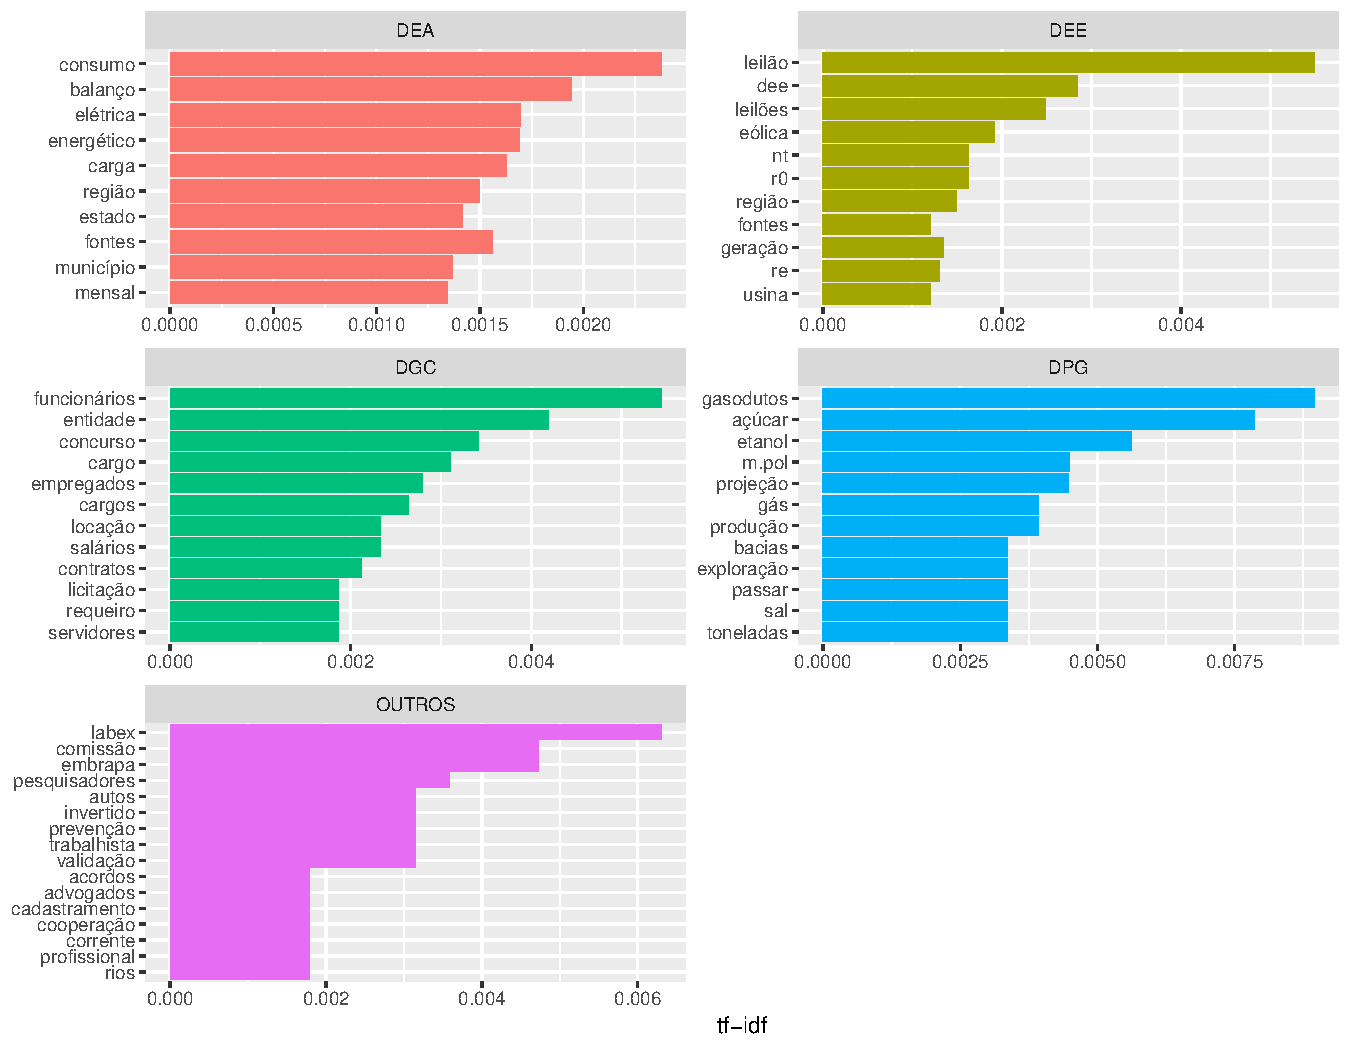
\includegraphics{markdown_v10_files/figure-latex/02_freq_palavras_dir-1.pdf}

\begin{Shaded}
\begin{Highlighting}[]
\CommentTok{#dev.off()}
\end{Highlighting}
\end{Shaded}

\paragraph{Filtrando um pedaço de
texto}\label{filtrando-um-pedaco-de-texto}

\begin{Shaded}
\begin{Highlighting}[]
\NormalTok{DB }\OperatorTok
\KeywordTok{filter}\NormalTok{(}\KeywordTok{str_detect}\NormalTok{(DESCRI_PEDIDO, }\StringTok{"r0"}\NormalTok{)) }\OperatorTok
\KeywordTok{select}\NormalTok{(DESCRI_PEDIDO) }\OperatorTok
\StringTok{  }\KeywordTok{head}\NormalTok{()}
\end{Highlighting}
\end{Shaded}

\begin{verbatim}
##                                                                                                                                                                                                                                                                                                                                                                                                                                                                                                                                                 DESCRI_PEDIDO
## 1                                                                                                                                                                                                                                                                          Prezados,\n\nSolicitamos que o deck do Newave 22.6 utilizado para Revisão da Garantia Física de UHEs, conforme consta da Nota Técnica EPE-DEE-RE-097/2016-r0 da Empresa de Pesquisa Energética -  EPE, nos seja enviado para conhecimento, por gentileza.\n\nObrigada,\nGraziella.
## 2                                                                                                                                                                                                                                                                                                                                                                                                                                                        Gostaria de ter acesso à Nota Técnica EPE-DEE-RE-097/2016-r0, pois não a encontro disponível online.
## 3 Solicitamos para nossa análise cópias dos relatórios nºs EPE-DEE-RE-147/2008-r0 que trata dos ESTUDOS RELATIVOS AOS GRANDES APROVEITAMENTOS HIDRELÉTRICOS NA REGIÃO AMAZÔNICA – Análise do sistema de atendimento aos estados do Acre e Rondônia no período Pré-Madeira – dezembro de 2008 e do relatório nº RE-EPES–4.010/08, que trata do SISTEMA ACRE-RONDÔNIA R2 – Estudos de Transitórios Eletromagnéticos e Condutor Econômico das LTs 230 kV P.Velho – Abunã – Rio Branco – janeiro de 2009.\n\nAgradecemos breve retorno.\n\nAtt.\n\nMônica\n\n\n\n
## 4                                                                                                                                                                                                                                                                                                                                                                            Cópia do documento EPE-DEE-RE-083/2010-r0, “Estudo de Integração das Usinas Hidrelétricas Previstas para o Estado de Santa Catarina”, elaborado pela EPE em novembro de 2010. \n
## 5                                                                                                                                                                                                                                                                                                                                                                                                                                                                                                       Solicito cópia da Nota Técnica EPE-DEE-RE-097/2016-r0
## 6                                                                                                                                                                                                                                                                                                                                                                                                          Bom dia, por gentileza gostaria ter acesso ao parecer técnico EPE-DEE-PT-051/2016-r0 e projeto alternativo apresentado pela tecnogera.\n\nObrigada
\end{verbatim}

Uma limpeza removendo palavras sem significado semântico
(\textbf{stopwords}) pode auxiliar o algoritmo a retornar palavras ainda
mais acertivas

\subsubsection{Radicais}\label{radicais}

Podemos diminuir redundâncias por parte do algoritmo ensinando-o a
compreender palavras que podem estar escritas de forma diferente mas que
em significado semântico são semelhantes. Para isso, analisamos o
radical de palavras com um mesmo prefixo mas com sufixos diferentes seja
por quisistos como gênero ou plural.

Exemplos:

leilão \(\propto\) leilões estado \(\propto\) estados região \(\propto\)
regiões

\texttt{Falta\ implementar}

\subsubsection{Stopwords}\label{stopwords}

\begin{Shaded}
\begin{Highlighting}[]
\NormalTok{FILE2 =}\StringTok{ "stopwords_PT_FINAL.csv"}
\NormalTok{stopwords_pt =}\StringTok{ }\KeywordTok{read.csv}\NormalTok{(}\KeywordTok{paste0}\NormalTok{(PATH,FILE2), }\DataTypeTok{sep =} \StringTok{';'}\NormalTok{, }\DataTypeTok{header =}\NormalTok{ F, }\DataTypeTok{encoding =} \StringTok{"UTF-8"}\NormalTok{)}
\NormalTok{stopwords_pt =}\StringTok{ }\NormalTok{stopwords_pt[,}\OperatorTok{-}\DecValTok{2}\NormalTok{]; }
\KeywordTok{cat}\NormalTok{(}\KeywordTok{paste0}\NormalTok{(}\StringTok{"O nosso vetor de stopwords contém "}\NormalTok{,}\KeywordTok{length}\NormalTok{(stopwords_pt), }\StringTok{" palavras únicas"}\NormalTok{))}
\end{Highlighting}
\end{Shaded}

\begin{verbatim}
## O nosso vetor de stopwords contém 562 palavras únicas
\end{verbatim}

\begin{Shaded}
\begin{Highlighting}[]
\NormalTok{## dim(stopwords_pt); class(stopwords_pt)}
\NormalTok{stopwords_pt =}\StringTok{ }\KeywordTok{as.character}\NormalTok{(stopwords_pt)}
\NormalTok{stopwords_pt[}\DecValTok{1}\OperatorTok{:}\DecValTok{14}\NormalTok{]}
\end{Highlighting}
\end{Shaded}

\begin{verbatim}
##  [1] "<U+FEFF>a" "à"       "acerca"  "adeus"   "agora"   "aí"      "ainda"  
##  [8] "alem"    "além"    "algmas"  "algo"    "algumas" "alguns"  "ali"
\end{verbatim}

\paragraph{\texorpdfstring{Freq. de palavras sem \textbf{stopwords} por
diretoria}{Freq. de palavras sem stopwords por diretoria}}\label{freq.-de-palavras-sem-stopwords-por-diretoria}

\begin{Shaded}
\begin{Highlighting}[]
\NormalTok{mystopwords <-}\StringTok{ }\KeywordTok{data_frame}\NormalTok{(}\DataTypeTok{palavra =}\NormalTok{ stopwords_pt)}
\end{Highlighting}
\end{Shaded}

\begin{verbatim}
## Warning: `data_frame()` is deprecated, use `tibble()`.
## This warning is displayed once per session.
\end{verbatim}

\begin{Shaded}
\begin{Highlighting}[]
\NormalTok{diretoria_palavras_noSTOP <-}\StringTok{ }\KeywordTok{anti_join}\NormalTok{(diretoria_palavras, mystopwords, }\DataTypeTok{by =} \StringTok{"palavra"}\NormalTok{)}
\CommentTok{#View(head(diretoria_palavras_noSTOP))}
\end{Highlighting}
\end{Shaded}

\begin{Shaded}
\begin{Highlighting}[]
\CommentTok{#diretoria_palavras_noSTOP_noSTOP}
\NormalTok{plot_diretoria_palavras_noSTOP <-}\StringTok{ }\NormalTok{diretoria_palavras_noSTOP }\OperatorTok
\StringTok{  }\KeywordTok{bind_tf_idf}\NormalTok{(palavra, DIRETORIA, n) }\OperatorTok
\StringTok{  }\KeywordTok{arrange}\NormalTok{(}\KeywordTok{desc}\NormalTok{(tf_idf)) }\OperatorTok
\StringTok{  }\KeywordTok{mutate}\NormalTok{(}\DataTypeTok{word =} \KeywordTok{factor}\NormalTok{(palavra, }\DataTypeTok{levels =} \KeywordTok{rev}\NormalTok{(}\KeywordTok{unique}\NormalTok{(palavra)))) }\OperatorTok
\StringTok{  }\KeywordTok{mutate}\NormalTok{(}\DataTypeTok{DIRETORIA =} \KeywordTok{factor}\NormalTok{(DIRETORIA, }\DataTypeTok{levels =} \KeywordTok{c}\NormalTok{(}\StringTok{"DEA"}\NormalTok{,}
                                                  \StringTok{"DEE"}\NormalTok{,}
                                                  \StringTok{"DGC"}\NormalTok{,}
                                                  \StringTok{"DPG"}\NormalTok{,}
                                                  \StringTok{"OUTROS"}\NormalTok{)))}
\CommentTok{#plot_diretoria_palavras_noSTOP}
\CommentTok{#windows.options(width=10, height=10)}
\CommentTok{#jpeg("03_freq_palavras_dir_nostop.jpeg")}
\NormalTok{plot_diretoria_palavras_noSTOP }\OperatorTok
\KeywordTok{group_by}\NormalTok{(DIRETORIA) }\OperatorTok
\KeywordTok{top_n}\NormalTok{(}\DecValTok{10}\NormalTok{, tf_idf) }\OperatorTok
\KeywordTok{ungroup}\NormalTok{() }\OperatorTok
\KeywordTok{mutate}\NormalTok{(}\DataTypeTok{palavra =} \KeywordTok{reorder}\NormalTok{(palavra, tf_idf)) }\OperatorTok
\KeywordTok{ggplot}\NormalTok{(}\KeywordTok{aes}\NormalTok{(palavra, tf_idf, }\DataTypeTok{fill =}\NormalTok{ DIRETORIA)) }\OperatorTok{+}
\KeywordTok{geom_col}\NormalTok{(}\DataTypeTok{show.legend =} \OtherTok{FALSE}\NormalTok{) }\OperatorTok{+}
\KeywordTok{labs}\NormalTok{(}\DataTypeTok{x =} \OtherTok{NULL}\NormalTok{, }\DataTypeTok{y =} \StringTok{"tf-idf"}\NormalTok{) }\OperatorTok{+}
\KeywordTok{facet_wrap}\NormalTok{(}\OperatorTok{~}\NormalTok{DIRETORIA, }\DataTypeTok{ncol =} \DecValTok{2}\NormalTok{, }\DataTypeTok{scales =} \StringTok{"free"}\NormalTok{) }\OperatorTok{+}
\KeywordTok{coord_flip}\NormalTok{()}
\end{Highlighting}
\end{Shaded}

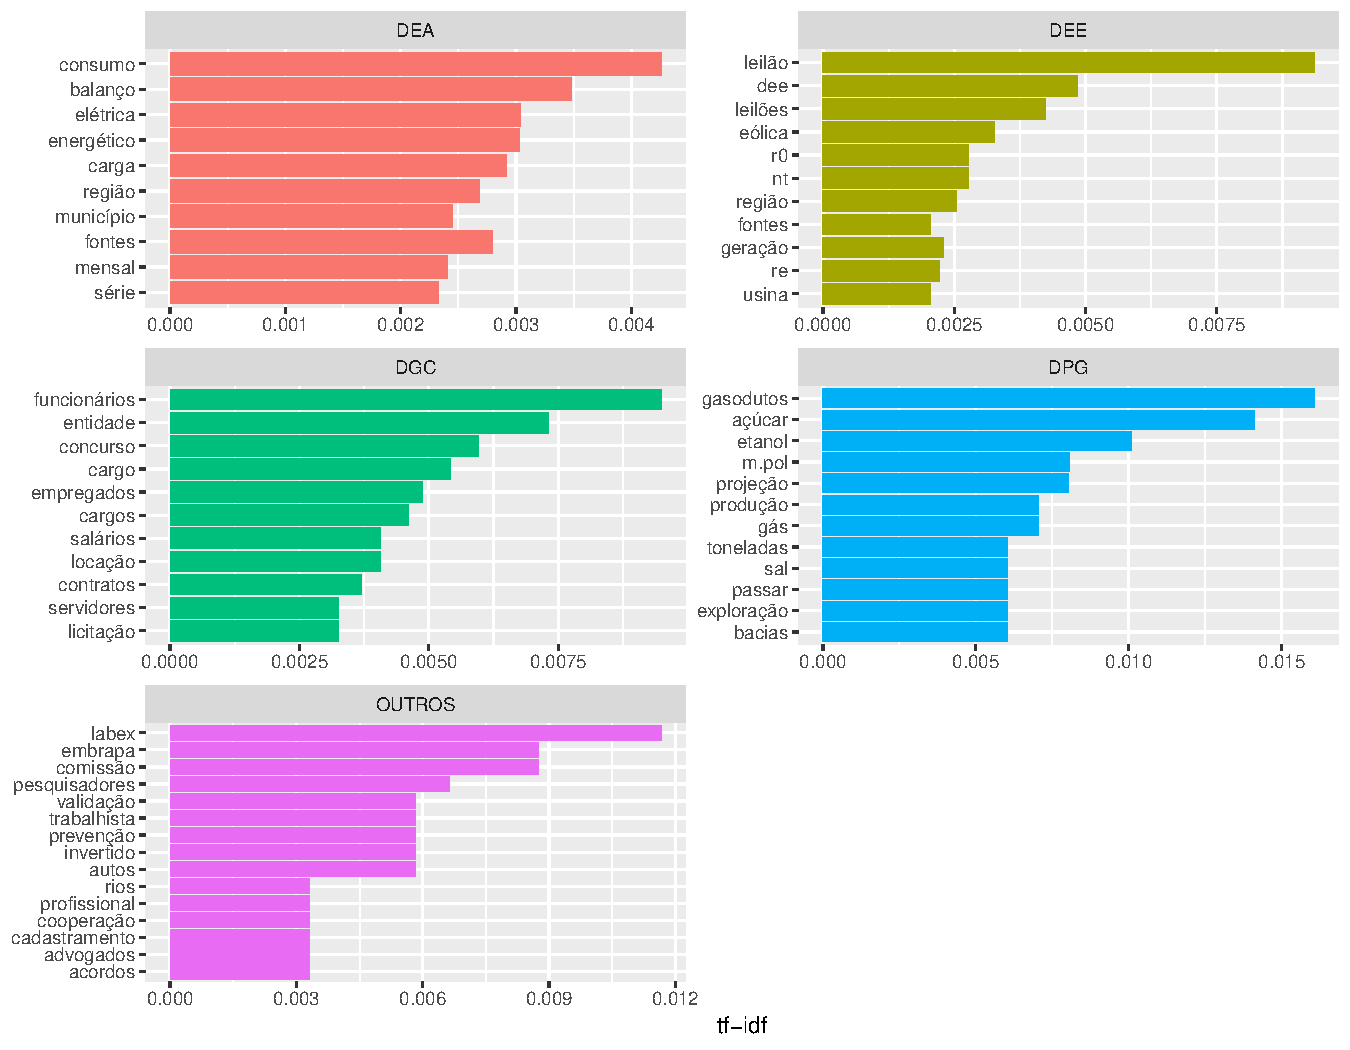
\includegraphics{markdown_v10_files/figure-latex/03_freq_palavras_dir_nostop-1.pdf}

\begin{Shaded}
\begin{Highlighting}[]
\CommentTok{#dev.off()}
\end{Highlighting}
\end{Shaded}


\end{document}
